\documentclass[class=article, crop=false]{standalone}
\usepackage{tikz}
\usepackage{subcaption}
\usetikzlibrary{calc}

\begin{document}

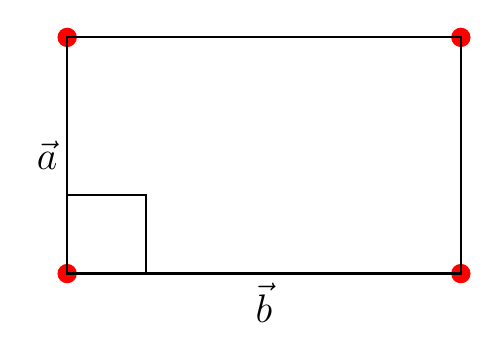
\begin{tikzpicture}
    \def\a{5}  % length of side a
    \def\b{3}  % length of side b
    \def\y{5}

    % Calculate the coordinates of the points
    \coordinate (A) at (0, 0);
    \coordinate (B) at (\a, 0);
    \coordinate (C) at (\a, \b);
    \coordinate (D) at (0, \b);

    %\coordinate (A2) at (0, 0 - \y);
    %\coordinate (B2) at (\a, 0- \y);
    %\coordinate (C2) at (\a, \b - \y);
    %\coordinate (D2) at (0, \b - \y);

    % Creates nodes at vertices
    \fill[red]  (A) circle(3.5pt) (B) circle(3.5pt) (C) circle(3.5pt) (D) circle(3.5pt);% (A2) circle(3.5pt) (B2) circle(3.5pt) (C2) circle(3.5pt) (D2) circle(3.5pt);
    %\fill[blue] ($(A2)!0.5!(C2)$) circle(3.5pt);

    % Draw right angle
    \draw[thick] (0,1) -- (1,1) -- (1,0);
    %\draw[thick] (0,1-\y) -- (1,1-\y) -- (1,0-\y);

    % Draw the rectangular unit cell
    \draw[thick] (A) -- (B) -- (C) -- (D) -- cycle;
    %\draw[thick] (A2) -- (B2) -- (C2) -- (D2) -- cycle;
    %\draw[dashed] (A2) -- (C2);
    %\draw[dashed] (B2) -- (D2);


    %Draw lattice parameters
    \node[left] at ($(A)!0.5!(D)$) {\Large $\vec{a}$};
    \node[below] at ($(A)!0.5!(B)$) {\Large $\vec{b}$};
    %\node[left] at ($(A2)!0.5!(D2)$) {\Large $\vec{a}$};
    %\node[below] at ($(A2)!0.5!(B2)$) {\Large $\vec{b}$};
    
\end{tikzpicture}
        
\end{document}